\section{Badanie wpływu szumu na proces uczenia}
\label{sec:szum}

Do tej pory, proces uczenia i~weryfikacji modeli przebiegał na niezaszumionych danych. W~przypadku danych rzeczywistych, przykładowo zebranych przez pewne urządzenie pomiarowe, rzadko kiedy mamy do czynienia z~taką sytuacją. W~ramach kolejnego eksperymentu, przetestowaliśmy jakość obliczonych w~sekcji~\ref{sec:optymalizacja} modeli. Na oryginalną funkcję nałożyliśmy biały, addytywny, gaussowski szum, zgodnie z~poniższym wzorem:

\begin{equation}
    f'(x,y) = f(x,y) + X \qquad X \sim \mathcal{N}(0, \sigma)\smallskip
\end{equation}

Wartości zmiennej losowej $X$ zostały obliczone przy użyciu funkcji \texttt{normal} z~modułu \texttt{numpy.random}.

W~ramach eksperymentu, sprawdzone zostało jak zmieniają się wskaźniki jakości przy rosnącej wartości parametru~$\sigma$. Dodatkowo, zależność jakości maszyny wektorów nośnych od poziomu szumu zostanie porównana z~jakością innego modelu. Celem tego porównania jest próba weryfikacji tezy, iż modele SVR są bardziej odporne na szum, w~porównaniu do innych modeli regresji. Do porównania został wykorzystany zwykły model regresji liniowej, który został zaimplementowany w~bibliotece \textbf{scikit-learn}~\cite{scikit-learn}.

\begin{lstlisting}[language=Python, captionpos=b, caption=Nagłówek klasy \texttt{LinearRegression}]
class linear_model.LinearRegression(*, 
    fit_intercept=True, 
    normalize=False, 
    copy_X=True, n_jobs=None, 
    positive=False)
\end{lstlisting}

\begin{figure}[h]
    \centering
    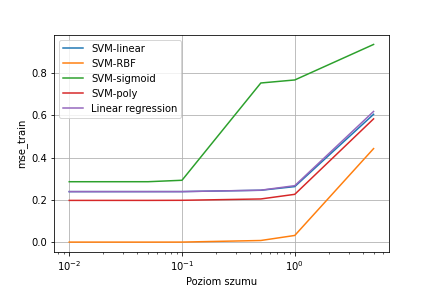
\includegraphics[width=1.1\columnwidth]{assets/mse_train.png}
    \caption{Wartość wskaźnika $MSE$ dla zbioru uczącego w~zależności od szumu}
    \label{fig:noise-mse-train}
\end{figure}

\begin{figure}[h]
    \centering
    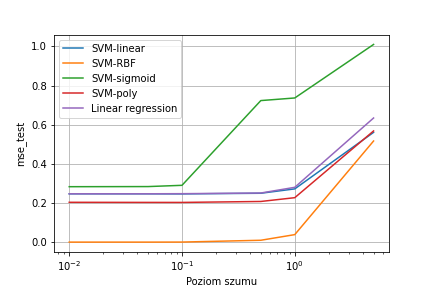
\includegraphics[width=1.1\columnwidth]{assets/mse_test.png}
    \caption{Wartość wskaźnika $MSE$ dla zbioru testowego w~zależności od szumu}
    \label{fig:noise-mse-test}
\end{figure}

%%%%%%%%%%%%%%%%%%%%%%%%%%%%%%%%%%%%%%%%%%%%%%%%%%%%%%%%%%%%%%%%%%%%%%%%%%%%%%%%

\begin{figure}[h]
    \centering
    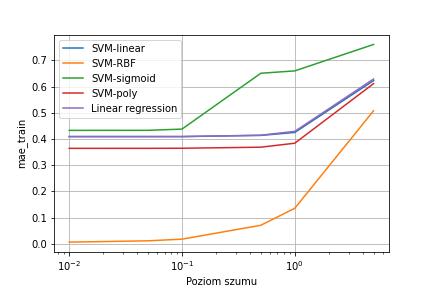
\includegraphics[width=1.1\columnwidth]{assets/mae_train.png}
    \caption{Wartość wskaźnika $MAE$ dla zbioru uczącego w~zależności od szumu}
    \label{fig:noise-mae-train}
\end{figure}

\begin{figure}[h]
    \centering
    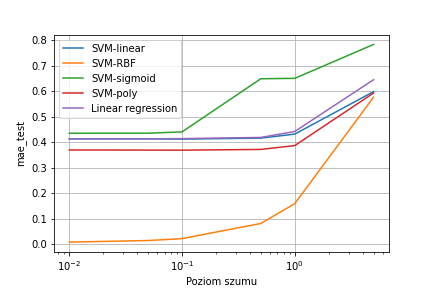
\includegraphics[width=1.1\columnwidth]{assets/mae_test.png}
    \caption{Wartość wskaźnika $MAE$ dla zbioru testowego w~zależności od szumu}
    \label{fig:noise-mae-test}
\end{figure}

%%%%%%%%%%%%%%%%%%%%%%%%%%%%%%%%%%%%%%%%%%%%%%%%%%%%%%%%%%%%%%%%%%%%%%%%%%%%%%%%

\begin{figure}[h]
    \centering
    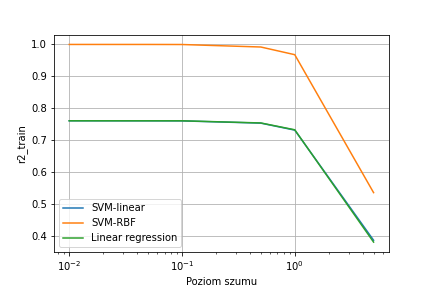
\includegraphics[width=1.1\columnwidth]{assets/r2_train.png}
    \caption{Wartość wskaźnika $R^2$ dla zbioru uczącego w~zależności od szumu}
    \label{fig:noise-r2-train}
\end{figure}

\begin{figure}[h]
    \centering
    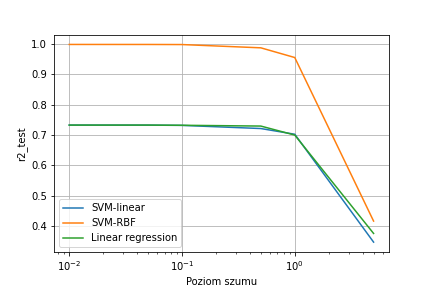
\includegraphics[width=1.1\columnwidth]{assets/r2_test.png}
    \caption{Wartość wskaźnika $R^2$ dla zbioru testowego w~zależności od szumu}
    \label{fig:noise-r2-test}
\end{figure}

Na rysunkach~\ref{fig:noise-mse-train}, \ref{fig:noise-mae-train} zostały przedstawione zależności trzech wskaźników jakości ($MSE$, $MAE$) od poziomu szumu $\sigma$ dla zbioru uczącego, a na rysunkach ~\ref{fig:noise-mse-test}, \ref{fig:noise-mae-test} odpowiednie zależności tych samych wskaźników dla zbioru testowego. Z problemem, niezależnie od poziomu szumu, zdecydowanie najgorzej poradził sobie SVM z sigmoidalną funkcją jądrową, co nie było zaskoczeniem ze względu na wyniki, które zostały zaprezentowane w \ref{sec:optymalizacja}. Dla tego typu modelu najszybciej wystąpiło znaczące pogorszenie wyników regresji. 

Zarówno dla $MSE$ jak i $MAE$ widać niezwykle podobieństwo osiąganych wyników pomiędzy maszyną wektorów nośnych o jądrze liniowym, a klasyczną regresją liniową. Różnica pomiędzy tymi modelami zaczyna być widoczna dla szumu rzędu jedności dla zbioru testowego z korzyścią dla SVR. Dla tych wskaźników niewiele gorzej wypadł SVM z wielomianową funkcją jądrową.

Zdecydowanie najlepiej z zadaniem uogólniania w zależności od szumu poradził sobie model maszyny wektorów nośnych z radialną funkcją jądrową. Warto tutaj jednak zauważyć, że dla szumu o $\sigma$ rzędu jedności to dla tego modelu występuje najbardziej gwałtowne pogorszenie wskaźników. 

Na rysunkach~\ref{fig:noise-r2-train}, oraz \ref{fig:noise-r2-test} zostały przedstawione zależności dla wskaźnika $R^2$ (determinacji) jedynie dla 3 modeli.  Dla SVM o funkcjach liniowych: sigmoidalnej i wielomianowej wyniki były na tyle złe ($R^2 < -2\times10^{5}$), że nie zostały tutaj zaprezentowane-- te modele nie radziły sobie z zaszumionymi danymi. Dla pozostałych modeli zależności pomiędzy jakością wyników regresji a szumem są podobne jak dla $MSE$ i $MAE$.
